%%% describe all the experiments performed and their statistical analysis
\chapter{Results} % at least 10, maximum 40 pages

%%%%%%%%%%%%%%%%%%%%%%%%%%%%%%%%%%%%%%%%%%%%%%%%%%%%%%%%%%%%%%%%%%%%%%%%%%%%%%%%
\section{Characterization of Physicochemical Properties}
  \subsection{Stacking Potential}
    \paragraph*{Obtaining the Datasets}\mbox{}\\
      A total of $83500$ protein structure files were downloaded from the PDB, some of which also contained ligands. Similarly, $3032$ structures with protein and nucleic acid complexes where downloaded, with the presence of ligands in some of them. From these two datasets, $22786$ unique ligand IDs were observed. The CIF files for these ligands were also downloaded from the PDB.

    \paragraph*{Detecting Aromatic Groups in Ligands}\mbox{}\\
      The first method of detection (parsing the SMILES strings) found aromaticity in $18211$ ligands from the dataset, while the second method (simple topological examination of the structures) found aromatic groups in $19096$ ligand files. From these ligands, $388$ were detected only by the first method, while $1273$ were detected only by the second method, meaning that the detection methods disagreed in the case of $1661$ ligands (figure \ref{fig:results/stacking}).

      \begin{figure}[H]
        \centering
        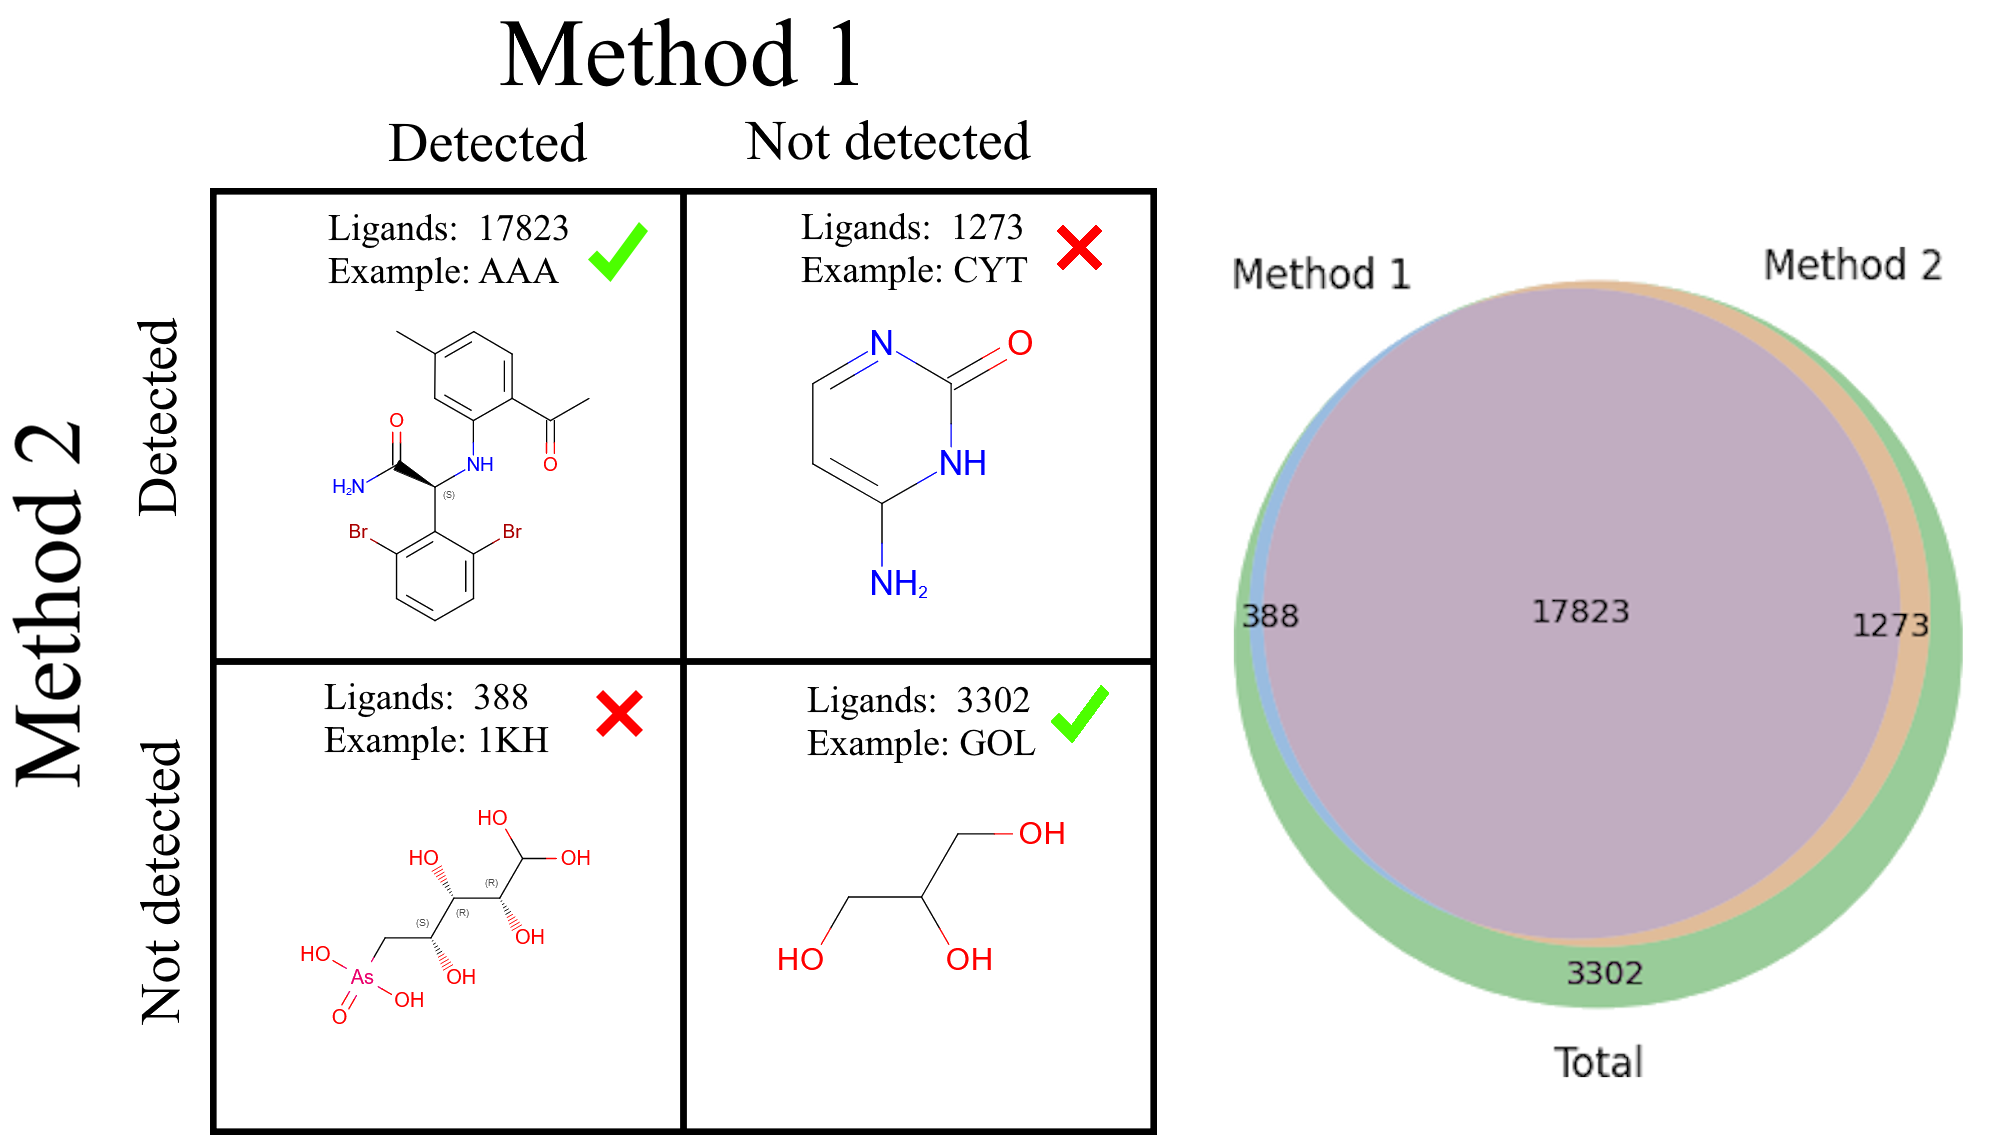
\includegraphics[width=0.8\textwidth]{figures/results/stacking.png}
        \caption{\label{fig:results/stacking} [TODO: description]}
      \end{figure}

      Some CIF files from the dataset had faulty SMILES strings (such as including the ligand name as a placeholder) or did not report correctly the aromaticity of the ligands. An example of the latter is the nucleic acid cytosine (CYT in figure \ref{fig:results/stacking}), which is not properly identified as aromatic despite being a classic example of a very biologically relevant aromatic group. This also was observed in uracyl and other pyrimidines.

      % 18211 method 1
      % 18404 method 2 --> should be more
      % 1273  detected only by method 2
      % 388   detected only by method 1

      The opposite situation also happened, where the SMILES string apparently contained aromatic atoms because lowercase symbols were found. However, this sometimes corresponded unrelated heavy atoms. An example of this occurance is the ligand 1KH in figure \ref{fig:results/stacking}, whose arsenic atom is represented by "As" in the SMILES string, so the first method recognized the lowercase "s" as an aromatic sulfur. The second method however immediatly discarded the ligand as it is acyclic.

      Some other instances with complex combinations of aromatic and non-aromatic rings (oftentimes connected by one or two atoms) presented problems for the second method, while being correctly reported in the first method (figure [TODO: add some examples in appendix\_ii]). For these reasons, these $1661$ were manually inspected to clarify whether aromaticity was present or not. At the end of this process, $18298$ ligands (accounting for $80.3 \% $ of the original dataset) were found to present a combined total of $34807$ aromatic groups (on average, 1.9 aromatic groups per ligand).

    \paragraph*{Sampling of Aromatic Interactions}\mbox{}\\
      a

      [TODO: statistical results from the dataset]

    \paragraph*{Model Definition}\mbox{}\\
      a

      [TODO: description of how the model shape was defined as a gaussian based in the histograms of distance and alpha angles, as well as its parameters mu and sigma]

      [TODO: show the donuts formed by the multivariate gaussian model]

  \subsection{Hydrogen Bonds Potential}
    [TODO: show the spheres formed by the univariate gaussian model]

    [TODO: description of the simultaneous positions where the ligand can have an ideal angle for the given distance]

  \subsection{Electrostatic Potential}
    [TODO: show the christmas tree effect and compare it to logAPBS]

    [TODO: show the log and trimmed log plots]


%%%%%%%%%%%%%%%%%%%%%%%%%%%%%%%%%%%%%%%%%%%%%%%%%%%%%%%%%%%%%%%%%%%%%%%%%%%%%%%%
\section{Development of Visualization Methods}
  \subsection{Graphical User Interface}
    % Pocket Sphere stuff
    [TODO: pocket sphere and changing its size vs pocket sphere off]

    [TODO: cartoon vs surface representation]

    [TODO: trimmed vs not trimmed sphere]

  \subsection{Potentials Visualization}
    % Representation of the potential grids in UnityMol
    [TODO: cloud vs isosurface]


%%%%%%%%%%%%%%%%%%%%%%%%%%%%%%%%%%%%%%%%%%%%%%%%%%%%%%%%%%%%%%%%%%%%%%%%%%%%%%%%
\section{Benchmarking}
  \subsection{Protein Systems}
    [TODO]

  \subsection{RNA Systems}
    [TODO]


%%%%%%%%%%%%%%%%%%%%%%%%%%%%%%%%%%%%%%%%%%%%%%%%%%%%%%%%%%%%%%%%%%%%%%%%%%%%%%%%
